              
                %% bare_jrnl.tex
%% V1.4b
%% 2015/08/26
%% by Michael Shell
%% see http://www.michaelshell.org/
%% for current contact information.
%%
%% This is a skeleton file demonstrating the use of IEEEtran.cls
%% (requires IEEEtran.cls version 1.8b or later) with an IEEE
%% journal paper.
%%
%% Support sites:
%% http://www.michaelshell.org/tex/ieeetran/
%% http://www.ctan.org/pkg/ieeetran
%% and
%% http://www.ieee.org/

%%*************************************************************************
%% Legal Notice:
%% This code is offered as-is without any warranty either expressed or
%% implied; without even the implied warranty of MERCHANTABILITY or
%% FITNESS FOR A PARTICULAR PURPOSE! 
%% User assumes all risk.
%% In no event shall the IEEE or any contributor to this code be liable for
%% any damages or losses, including, but not limited to, incidental,
%% consequential, or any other damages, resulting from the use or misuse
%% of any information contained here.
%%
%% All comments are the opinions of their respective authors and are not
%% necessarily endorsed by the IEEE.
%%
%% This work is distributed under the LaTeX Project Public License (LPPL)
%% ( http://www.latex-project.org/ ) version 1.3, and may be freely used,
%% distributed and modified. A copy of the LPPL, version 1.3, is included
%% in the base LaTeX documentation of all distributions of LaTeX released
%% 2003/12/01 or later.
%% Retain all contribution notices and credits.
%% ** Modified files should be clearly indicated as such, including  **
%% ** renaming them and changing author support contact information. **
%%*************************************************************************


% *** Authors should verify (and, if needed, correct) their LaTeX system  ***
% *** with the testflow diagnostic prior to trusting their LaTeX platform ***
% *** with production work. The IEEE's font choices and paper sizes can   ***
% *** trigger bugs that do not appear when using other class files.       ***                          ***
% The testflow support page is at:
% http://www.michaelshell.org/tex/testflow/


% Please refer to your journal's instructions for other
% options that should be set.
\documentclass[journal,onecolumn]{IEEEtran}
% \documentclass{article}
% If IEEEtran.cls has not been installed into the LaTeX system files,
% manually specify the path to it like:
% \documentclass[journal]{../sty/IEEEtran}

\usepackage{amsmath} 
\usepackage{graphicx} 
\usepackage{hyperref}
\usepackage{caption}


\usepackage{tabularx} % for the 'tabularx' environment
\usepackage{booktabs} 



% Some very useful LaTeX packages include:
% (uncomment the ones you want to load)


% *** MISC UTILITY PACKAGES ***
%
%\usepackage{ifpdf}
% Heiko Oberdiek's ifpdf.sty is very useful if you need conditional
% compilation based on whether the output is pdf or dvi.
% usage:
% \ifpdf
%   % pdf code
% \else
%   % dvi code
% \fi
% The latest version of ifpdf.sty can be obtained from:
% http://www.ctan.org/pkg/ifpdf
% Also, note that IEEEtran.cls V1.7 and later provides a builtin
% \ifCLASSINFOpdf conditional that works the same way.
% When switching from latex to pdflatex and vice-versa, the compiler may
% have to be run twice to clear warning/error messages.






% *** CITATION PACKAGES ***
%
%\usepackage{cite}
% cite.sty was written by Donald Arseneau
% V1.6 and later of IEEEtran pre-defines the format of the cite.sty package
% \cite{} output to follow that of the IEEE. Loading the cite package will
% result in citation numbers being automatically sorted and properly
% "compressed/ranged". e.g., [1], [9], [2], [7], [5], [6] without using
% cite.sty will become [1], [2], [5]--[7], [9] using cite.sty. cite.sty's
% \cite will automatically add leading space, if needed. Use cite.sty's
% noadjust option (cite.sty V3.8 and later) if you want to turn this off
% such as if a citation ever needs to be enclosed in parenthesis.
% cite.sty is already installed on most LaTeX systems. Be sure and use
% version 5.0 (2009-03-20) and later if using hyperref.sty.
% The latest version can be obtained at:
% http://www.ctan.org/pkg/cite
% The documentation is contained in the cite.sty file itself.



\usepackage{array} % for the 'p' column type


% *** GRAPHICS RELATED PACKAGES ***
%
\ifCLASSINFOpdf
  \usepackage[pdftex]{graphicx}
  % declare the path(s) where your graphic files are
  % \graphicspath{{../pdf/}{../jpeg/}}
  % and their extensions so you won't have to specify these with
  % every instance of \includegraphics
  % \DeclareGraphicsExtensions{.pdf,.jpeg,.png}
\else
  % or other class option (dvipsone, dvipdf, if not using dvips). graphicx
  % will default to the driver specified in the system graphics.cfg if no
  % driver is specified.
  % \usepackage[dvips]{graphicx}
  % declare the path(s) where your graphic files are
  % \graphicspath{{../eps/}}
  % and their extensions so you won't have to specify these with
  % every instance of \includegraphics
  % \DeclareGraphicsExtensions{.eps}
\fi
% graphicx was written by David Carlisle and Sebastian Rahtz. It is
% required if you want graphics, photos, etc. graphicx.sty is already
% installed on most LaTeX systems. The latest version and documentation
% can be obtained at: 
% http://www.ctan.org/pkg/graphicx
% Another good source of documentation is "Using Imported Graphics in
% LaTeX2e" by Keith Reckdahl which can be found at:
% http://www.ctan.org/pkg/epslatex
%
% latex, and pdflatex in dvi mode, support graphics in encapsulated
% postscript (.eps) format. pdflatex in pdf mode supports graphics
% in .pdf, .jpeg, .png and .mps (metapost) formats. Users should ensure
% that all non-photo figures use a vector format (.eps, .pdf, .mps) and
% not a bitmapped formats (.jpeg, .png). The IEEE frowns on bitmapped formats
% which can result in "jaggedy"/blurry rendering of lines and letters as
% well as large increases in file sizes.
%
% You can find documentation about the pdfTeX application at:
% http://www.tug.org/applications/pdftex





% *** MATH PACKAGES ***
%
%\usepackage{amsmath}
% A popular package from the American Mathematical Society that provides
% many useful and powerful commands for dealing with mathematics.
%
% Note that the amsmath package sets \interdisplaylinepenalty to 10000
% thus preventing page breaks from occurring within multiline equations. Use:
%\interdisplaylinepenalty=2500
% after loading amsmath to restore such page breaks as IEEEtran.cls normally
% does. amsmath.sty is already installed on most LaTeX systems. The latest
% version and documentation can be obtained at:
% http://www.ctan.org/pkg/amsmath





% *** SPECIALIZED LIST PACKAGES ***
%
%\usepackage{algorithmic}
% algorithmic.sty was written by Peter Williams and Rogerio Brito.
% This package provides an algorithmic environment fo describing algorithms.
% You can use the algorithmic environment in-text or within a figure
% environment to provide for a floating algorithm. Do NOT use the algorithm
% floating environment provided by algorithm.sty (by the same authors) or
% algorithm2e.sty (by Christophe Fiorio) as the IEEE does not use dedicated
% algorithm float types and packages that provide these will not provide
% correct IEEE style captions. The latest version and documentation of
% algorithmic.sty can be obtained at:
% http://www.ctan.org/pkg/algorithms
% Also of interest may be the (relatively newer and more customizable)
% algorithmicx.sty package by Szasz Janos:
% http://www.ctan.org/pkg/algorithmicx




% *** ALIGNMENT PACKAGES ***
%
\usepackage{array}
% Frank Mittelbach's and David Carlisle's array.sty patches and improves
% the standard LaTeX2e array and tabular environments to provide better
% appearance and additional user controls. As the default LaTeX2e table
% generation code is lacking to the point of almost being broken with
% respect to the quality of the end results, all users are strongly
% advised to use an enhanced (at the very least that provided by array.sty)
% set of table tools. array.sty is already installed on most systems. The
% latest version and documentation can be obtained at:
% http://www.ctan.org/pkg/array


% IEEEtran contains the IEEEeqnarray family of commands that can be used to
% generate multiline equations as well as matrices, tables, etc., of high
% quality.




% *** SUBFIGURE PACKAGES ***
%\ifCLASSOPTIONcompsoc
%  \usepackage[caption=false,font=normalsize,labelfont=sf,textfont=sf]{subfig}
%\else
%  \usepackage[caption=false,font=footnotesize]{subfig}
%\fi
% subfig.sty, written by Steven Douglas Cochran, is the modern replacement
% for subfigure.sty, the latter of which is no longer maintained and is
% incompatible with some LaTeX packages including fixltx2e. However,
% subfig.sty requires and automatically loads Axel Sommerfeldt's caption.sty
% which will override IEEEtran.cls' handling of captions and this will result
% in non-IEEE style figure/table captions. To prevent this problem, be sure
% and invoke subfig.sty's "caption=false" package option (available since
% subfig.sty version 1.3, 2005/06/28) as this is will preserve IEEEtran.cls
% handling of captions.
% Note that the Computer Society format requires a larger sans serif font
% than the serif footnote size font used in traditional IEEE formatting
% and thus the need to invoke different subfig.sty package options depending
% on whether compsoc mode has been enabled.
%
% The latest version and documentation of subfig.sty can be obtained at:
% http://www.ctan.org/pkg/subfig




% *** FLOAT PACKAGES ***
%
%\usepackage{fixltx2e}
% fixltx2e, the successor to the earlier fix2col.sty, was written by
% Frank Mittelbach and David Carlisle. This package corrects a few problems
% in the LaTeX2e kernel, the most notable of which is that in current
% LaTeX2e releases, the ordering of single and double column floats is not
% guaranteed to be preserved. Thus, an unpatched LaTeX2e can allow a
% single column figure to be placed prior to an earlier double column
% figure.
% Be aware that LaTeX2e kernels dated 2015 and later have fixltx2e.sty's
% corrections already built into the system in which case a warning will
% be issued if an attempt is made to load fixltx2e.sty as it is no longer
% needed.
% The latest version and documentation can be found at:
% http://www.ctan.org/pkg/fixltx2e


%\usepackage{stfloats}
% stfloats.sty was written by Sigitas Tolusis. This package gives LaTeX2e
% the ability to do double column floats at the bottom of the page as well
% as the top. (e.g., "\begin{figure*}[!b]" is not normally possible in
% LaTeX2e). It also provides a command:
%\fnbelowfloat
% to enable the placement of footnotes below bottom floats (the standard
% LaTeX2e kernel puts them above bottom floats). This is an invasive package
% which rewrites many portions of the LaTeX2e float routines. It may not work
% with other packages that modify the LaTeX2e float routines. The latest
% version and documentation can be obtained at:
% http://www.ctan.org/pkg/stfloats
% Do not use the stfloats baselinefloat ability as the IEEE does not allow
% \baselineskip to stretch. Authors submitting work to the IEEE should note
% that the IEEE rarely uses double column equations and that authors should try
% to avoid such use. Do not be tempted to use the cuted.sty or midfloat.sty
% packages (also by Sigitas Tolusis) as the IEEE does not format its papers in
% such ways.
% Do not attempt to use stfloats with fixltx2e as they are incompatible.
% Instead, use Morten Hogholm'a dblfloatfix which combines the features
% of both fixltx2e and stfloats:
%
% \usepackage{dblfloatfix}
% The latest version can be found at:
% http://www.ctan.org/pkg/dblfloatfix



%\ifCLASSOPTIONcaptionsoff
%  \usepackage[nomarkers]{endfloat}
% \let\MYoriglatexcaption\caption
% \renewcommand{\caption}[2][\relax]{\MYoriglatexcaption[#2]{#2}}
%\fi
% endfloat.sty was written by James Darrell McCauley, Jeff Goldberg and 
% Axel Sommerfeldt. This package may be useful when used in conjunction with 
% IEEEtran.cls'  captionsoff option. Some IEEE journals/societies require that
% submissions have lists of figures/tables at the end of the paper and that
% figures/tables without any captions are placed on a page by themselves at
% the end of the document. If needed, the draftcls IEEEtran class option or
% \CLASSINPUTbaselinestretch interface can be used to increase the line
% spacing as well. Be sure and use the nomarkers option of endfloat to
% prevent endfloat from "marking" where the figures would have been placed
% in the text. The two hack lines of code above are a slight modification of
% that suggested by in the endfloat docs (section 8.4.1) to ensure that
% the full captions always appear in the list of figures/tables - even if
% the user used the short optional argument of \caption[]{}.
% IEEE papers do not typically make use of \caption[]'s optional argument,
% so this should not be an issue. A similar trick can be used to disable
% captions of packages such as subfig.sty that lack options to turn off
% the subcaptions:
% For subfig.sty:
% \let\MYorigsubfloat\subfloat
% \renewcommand{\subfloat}[2][\relax]{\MYorigsubfloat[]{#2}}
% However, the above trick will not work if both optional arguments of
% the \subfloat command are used. Furthermore, there needs to be a
% description of each subfigure *somewhere* and endfloat does not add
% subfigure captions to its list of figures. Thus, the best approach is to
% avoid the use of subfigure captions (many IEEE journals avoid them anyway)
% and instead reference/explain all the subfigures within the main caption.
% The latest version of endfloat.sty and its documentation can obtained at:
% http://www.ctan.org/pkg/endfloat
%
% The IEEEtran \ifCLASSOPTIONcaptionsoff conditional can also be used
% later in the document, say, to conditionally put the References on a 
% page by themselves.




% *** PDF, URL AND HYPERLINK PACKAGES ***
%
%\usepackage{url}
% url.sty was written by Donald Arseneau. It provides better support for
% handling and breaking URLs. url.sty is already installed on most LaTeX
% systems. The latest version and documentation can be obtained at:
% http://www.ctan.org/pkg/url
% Basically, \url{my_url_here}.




% *** Do not adjust lengths that control margins, column widths, etc. ***
% *** Do not use packages that alter fonts (such as pslatex).         ***
% There should be no need to do such things with IEEEtran.cls V1.6 and later.
% (Unless specifically asked to do so by the journal or conference you plan
% to submit to, of course. )


% correct bad hyphenation here
\hyphenation{op-tical net-works semi-conduc-tor}


\begin{document}
%
% paper title
% Titles are generally capitalized except for words such as a, an, and, as,
% at, but, by, for, in, nor, of, on, or, the, to and up, which are usually
% not capitalized unless they are the first or last word of the title.
% Linebreaks \\ can be used within to get better formatting as desired.
% Do not put math or special symbols in the title.
\title{Designing Functional CQI Modules for OBE: A Driver-Barrier Analysis and Iterative Design Approach}
%
%
% author names and IEEE memberships
% note positions of commas and nonbreaking spaces ( ~ ) LaTeX will not break
% a structure at a ~ so this keeps an author's name from being broken across
% two lines.
% use \thanks{} to gain access to the first footnote area
% a separate \thanks must be used for each paragraph as LaTeX2e's \thanks
% was not built to handle multiple paragraphs
%

\author{Rashedul Amin Tuhin  and Dr. A.B.M. Alim Al Islam% <-this % stops a space
\thanks{}% <-this % stops a space
\thanks{}% <-this % stops a space
\thanks{}}

% note the % following the last \IEEEmembership and also \thanks - 
% these prevent an unwanted space from occurring between the last author name
% and the end of the author line. i.e., if you had this:
% 
% \author{....lastname \thanks{...} \thanks{...} }
%                     ^------------^------------^----Do not want these spaces!
%
% a space would be appended to the last name and could cause every name on that
% line to be shifted left slightly. This is one of those "LaTeX things". For
% instance, "\textbf{A} \textbf{B}" will typeset as "A B" not "AB". To get
% "AB" then you have to do: "\textbf{A}\textbf{B}"
% \thanks is no different in this regard, so shield the last } of each \thanks
% that ends a line with a % and do not let a space in before the next \thanks.
% Spaces after \IEEEmembership other than the last one are OK (and needed) as
% you are supposed to have spaces between the names. For what it is worth,
% this is a minor point as most people would not even notice if the said evil
% space somehow managed to creep in.



% The paper headers
\markboth{}%
{}
% The only time the second header will appear is for the odd numbered pages
% after the title page when using the twoside option.
% 
% *** Note that you probably will NOT want to include the author's ***
% *** name in the headers of peer review papers.                   ***
% You can use \ifCLASSOPTIONpeerreview for conditional compilation here if
% you desire.




% If you want to put a publisher's ID mark on the page you can do it like
% this:
%\IEEEpubid{0000--0000/00\$00.00~\copyright~2015 IEEE}
% Remember, if you use this you must call \IEEEpubidadjcol in the second
% column for its text to clear the IEEEpubid mark.



% use for special paper notices
%\IEEEspecialpapernotice{(Invited Paper)}




% make the title area
\maketitle

% As a general rule, do not put math, special symbols or citations
% in the abstract or keywords.
\begin{abstract}
Outcome Based Education (OBE) has been in practice for about a decade in Bangladesh and has been adopted to benchmark the quality of education by the University Grants Commission and the Board of Accreditation for Engineering and Technical Education (BAETE). The process and practices of OBE varies from one organization, because not having a specific guideline. Assistive technology has been proven to be useful for OBE practitioner institutions as a guide through the whole process. In this study, a number of drivers and barriers have been identified by interviewing two expert faculty members, and thematic analysis was performed to highlight the perceived drivers and barriers. Based on the strategic recommendations, several pseudo user interfaces were designed iteratively by collecting feedback from seven participants from different organizations. Based on the feedback, a number of design choices were made, and argued that such design choices would facilitate the goal of the CQI module, a subpart of the OBE software. The findings were reviewed by the participants and the design choices were adjusted to reflect the recommendations.
\end{abstract}

\begin{IEEEkeywords}
\textbf{\textit{Outcome Based Education, Institutional Perspective, OBE Software, Accessibility, CQI}}
\end{IEEEkeywords}







\IEEEpeerreviewmaketitle



\section{\textbf{Introduction}}
% The very first letter is a 2 line initial drop letter followed
% by the rest of the first word in caps.
% 
% form to use if the first word consists of a single letter:
% \IEEEPARstart{A}{demo} file is ....
% 
% form to use if you need the single drop letter followed by
% normal text (unknown if ever used by the IEEE):
% \IEEEPARstart{A}{}demo file is ....
% 
% Some journals put the first two words in caps:
% \IEEEPARstart{T}{his demo} file is ....
% 
% Here we have the typical use of a "T" for an initial drop letter
% and "HIS" in caps to complete the first word.
\IEEEPARstart{T}{he} accreditation requirements from the \textit{Board of Accreditation of Engineering and Technical Education (BAETE)}, and demand from the \textit{University Grants Commission (UGC)} of submitting a revised curriculum of different programs in tertiary level of education, forced the adaptation of \textit{Outcome Based Education (OBE)} to majority of the universities in Bangladesh. In contrast with the traditional education system, OBE focuses on enhancing the abilities of the students, which are termed as “\textit{Outcomes}”. The outcomes are often measured quantitatively at different levels, starting from lesson, topic, Course, Program ending at mission and vision, by using diverse assessment tools and techniques. The outcomes are aggregated quantitatively towards the measurement of outcomes at different levels. Figure \ref{fig:quntitative} exhibits a general aggregation of Topic Learning Outcomes (TO) to Course Learning Outcomes (CO) to Program Outcomes (PO) to Program Educational Objectives (PEO).

\begin{figure}
    \centering
    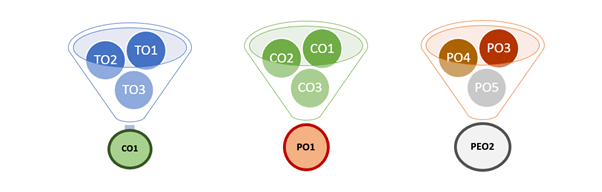
\includegraphics[width=1\linewidth]{img/Picture1.png}
    \caption{Quantitative aggregation of outcomes}
    \label{fig:quntitative}
\end{figure}


In tertiary level education, the integration of Outcome-Based Education (OBE) is driving the development of outcomes measurement software, a transformative tool emphasizing measurable student outcomes. This process is propelled by institutional commitments to fostering a culture of continuous improvement, bolstered by robust technological infrastructure and faculty engagement. However, the journey is not without challenges. Financial constraints often hinder investment in sophisticated software and comprehensive training, while technological challenges and resistance to change may disrupt seamless integration.  

A critical barrier lies in the lack of awareness or understanding about the benefits of such software, and institutional resistance rooted in cultural norms. Moreover, adhering to regulatory and accreditation requirements becomes a driver, ensuring institutions comply with educational standards. Multiple stakeholders, including students, teachers, administrators, alumni, employers, sponsors, and software developers, bring diverse perspectives and needs, further complicating the development and implementation process. Balancing these varied interests is essential for successful outcomes measurement software integration.  

In this complex landscape, educational software development faces the challenge of navigating evolving technologies, financial constraints, and the need for cultural shifts within institutions. Bridging the gap between traditional educational methods and innovative technologies requires careful consideration of stakeholder perspectives and the intricacies of institutional dynamics. Ultimately, the success of outcomes measurement software hinges on overcoming barriers, fostering collaboration among stakeholders, and aligning technological advancements with the diverse demands of the higher education landscape.

The remainder of this article are organized as follows: Section 2 would provide an overview of the theoretical frameworks of Outcome Based Education (OBE) and User Acceptance. The following sections would provide the context of the research problem, i.e., the history and practice of OBE in Bangladesh and define the scope of the project, followed by the research objectives as contributions. Section 4 and 5 comprehensively discuss the relevant literature, ontology and epistemology to methodology. Section 6 presents the findings and the interpretations and implications of the findings are discussed in the later section.






% An example of a floating figure using the graphicx package.
% Note that \label must occur AFTER (or within) \caption.
% For figures, \caption should occur after the \includegraphics.
% Note that IEEEtran v1.7 and later has special internal code that
% is designed to preserve the operation of \label within \caption
% even when the captionsoff option is in effect. However, because
% of issues like this, it may be the safest practice to put all your
% \label just after \caption rather than within \caption{}.
%
% Reminder: the "draftcls" or "draftclsnofoot", not "draft", class
% option should be used if it is desired that the figures are to be
% displayed while in draft mode.
%
%\begin{figure}[!t]
%\centering
%\includegraphics[width=2.5in]{myfigure}
% where an .eps filename suffix will be assumed under latex, 
% and a .pdf suffix will be assumed for pdflatex; or what has been declared
% via \DeclareGraphicsExtensions.
%\caption{Simulation results for the network.}
%\label{fig_sim}
%\end{figure}

% Note that the IEEE typically puts floats only at the top, even when this
% results in a large percentage of a column being occupied by floats.


% An example of a double column floating figure using two subfigures.
% (The subfig.sty package must be loaded for this to work.)
% The subfigure \label commands are set within each subfloat command,
% and the \label for the overall figure must come after \caption.
% \hfil is used as a separator to get equal spacing.
% Watch out that the combined width of all the subfigures on a 
% line do not exceed the text width or a line break will occur.
%
%\begin{figure*}[!t]
%\centering
%\subfloat[Case I]{\includegraphics[width=2.5in]{box}%
%\label{fig_first_case}}
%\hfil
%\subfloat[Case II]{\includegraphics[width=2.5in]{box}%
%\label{fig_second_case}}
%\caption{Simulation results for the network.}
%\label{fig_sim}
%\end{figure*}
%
% Note that often IEEE papers with subfigures do not employ subfigure
% captions (using the optional argument to \subfloat[]), but instead will
% reference/describe all of them (a), (b), etc., within the main caption.
% Be aware that for subfig.sty to generate the (a), (b), etc., subfigure
% labels, the optional argument to \subfloat must be present. If a
% subcaption is not desired, just leave its contents blank,
% e.g., \subfloat[].


% An example of a floating table. Note that, for IEEE style tables, the
% \caption command should come BEFORE the table and, given that table
% captions serve much like titles, are usually capitalized except for words
% such as a, an, and, as, at, but, by, for, in, nor, of, on, or, the, to
% and up, which are usually not capitalized unless they are the first or
% last word of the caption. Table text will default to \footnotesize as
% the IEEE normally uses this smaller font for tables.
% The \label must come after \caption as always.
%
%\begin{table}[!t]
%% increase table row spacing, adjust to taste
%\renewcommand{\arraystretch}{1.3}
% if using array.sty, it might be a good idea to tweak the value of
% \extrarowheight as needed to properly center the text within the cells
%\caption{An Example of a Table}
%\label{table_example}
%\centering
%% Some packages, such as MDW tools, offer better commands for making tables
%% than the plain LaTeX2e tabular which is used here.
%\begin{tabular}{|c||c|}
%\hline
%One & Two\\
%\hline
%Three & Four\\
%\hline
%\end{tabular}
%\end{table}


% Note that the IEEE does not put floats in the very first column
% - or typically anywhere on the first page for that matter. Also,
% in-text middle ("here") positioning is typically not used, but it
% is allowed and encouraged for Computer Society conferences (but
% not Computer Society journals). Most IEEE journals/conferences use
% top floats exclusively. 
% Note that, LaTeX2e, unlike IEEE journals/conferences, places
% footnotes above bottom floats. This can be corrected via the
% \fnbelowfloat command of the stfloats package.





\section{\textbf{Background}}
Outcome-Based Education (OBE) has become a key paradigm in the educational landscape, emphasizing measurable results and continuous improvement. In the context of undergraduate engineering education in Bangladesh, there is a growing need for an outcomes measurement software to enhance assessment, feedback, and overall program effectiveness.

\subsection{Theoretical Description of the user acceptance frameworks}

\subsubsection{Technology Acceptance Model (TAM, TAM+, TAM2, TAM3)}

The Technology Acceptance Model (TAM) predicts how likely people will use a new technology. It focuses on two main ideas: how useful people believe the technology is (Perceived Usefulness) and how easy they think it will be to use (Perceived Ease of use) \cite{adams_perceived_1992}. These two factors influence people's overall impression (Behavioral Intention), which ultimately leads to them using the technology or not. Other things, like what other people think (External Variables), can also affect how people feel about using a new technology. Figure\ref{fig:TAM} provides an overview of the TAM.

TAM has been improved over time to consider more factors. Newer versions include TAM+, TAM2, and TAM3, which take into account things like social pressure, how much control users feel they have, and if the technology fits with what they already do \cite{venkatesh_theoretical_2000}. Criticisms against TAM is that it doesn't fully explain why people use technology in all situations. To address this, there are even more advanced models that include things like emotions, how well-designed a system is, and how risky it seems to use. These models aim to give the most accurate picture possible of how people decide whether or not to use new technologies.
\begin{figure}[b]
    \centering
    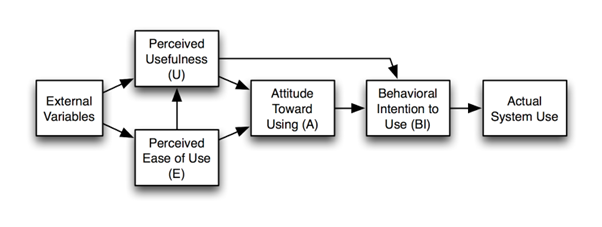
\includegraphics[width=1\linewidth]{img/Picture2.png}
    \caption{Technology Acceptance Model (TAM) }
    \label{fig:TAM}
\end{figure}

\subsubsection{Unified Theory of Acceptance and Use of Technology (UTAUT)}
The Unified Theory of Acceptance and Use of Technology (UTAUT) is a widely recognized framework in the field of information systems and technology acceptance research. Developed by Venkatesh et al., UTAUT integrates elements from eight existing technology acceptance models to provide a comprehensive understanding of user acceptance and adoption of technology. It identifies four key determinants of technology acceptance: performance expectancy, effort expectancy, social influence, and facilitating conditions. UTAUT has been extensively used to study and predict user behaviors related to the adoption of various technologies in different contexts.  

UTAUT explains how people use information systems and technology innovations. UTAUT \cite{venkatesh_user_2003}, combines ideas from TAM and other models to give an even more complete picture of why people use technology. UTAUT considers things like how well a technology works, how much effort it takes to learn, and whether people have the resources they need to use it \cite{ayaz_analysis_2020}.
\begin{figure}[t]
    \centering
    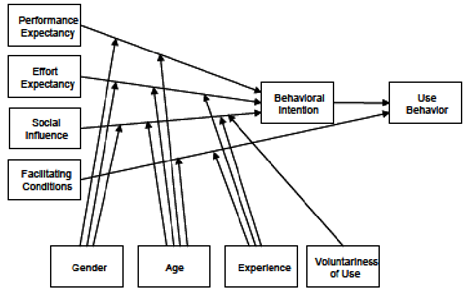
\includegraphics[width=0.8\linewidth]{img/Picture3.png}
    \caption{Unified Theory of Acceptance and Use of Technology (UTAUT) }
    \label{fig:utaut}
\end{figure}

\subsubsection{Other theoretical perspectives}
\vspace{12pt}
The \textit{Social Cognitive Theory (SCT)} \cite{10.1371/journal.pone.0134977}and \textit{Self-Determination Theory (SDT)} \cite{Law2020} provide a framework for understanding the psychological aspects of software development. SCT's emphasis on observational learning and self-efficacy can be directly applied to the way software developers learn from mentors and peers, assimilating new information and skills that are critical for their professional growth. Meanwhile, SDT's focus on intrinsic motivation underscores the importance of a supportive work environment that nurtures autonomy, competence, and relatedness. In practice, this could translate into giving developers the freedom to innovate, opportunities to tackle challenging projects, and fostering a sense of community within the team. These theories offer a comprehensive approach to enhancing the motivation, learning, and overall well-being of software developers, leading to more effective and innovative software development practices.

\vspace{12pt}


The \textit{Matching Person \& Technology (MPT)} model offers a person-centered framework for selecting and implementing assistive technology (AT). This user-driven approach emphasizes individual characteristics and needs to ensure optimal technology matching and successful adoption. The MPT process utilizes a comprehensive assessment of factors to evaluate a user's strengths, needs, preferences, psychosocial characteristics, and environmental factors \cite{scherer_matching_2017}. This multi-faceted approach helps distinguish potential technology users from non-users, leading to more effective technology selection across various domains including education, workplace, home, healthcare, mobility, and daily activities. However, a key challenge associated with the MPT model lies in accurately capturing user preferences \cite{scherer_matching_2002}. Due to their subjective nature, preferences can exhibit significant individual variability, potentially impacting the assessment's effectiveness.

\subsection{\textbf{History of OBE in Bangladesh}}
The \textit{International Professional Engineers Agreement (IPEA)}, formerly called the \textit{Engineers Mobility Forum (EMF)}, is a global accord between engineering bodies. It sets the stage for a unified international standard of professional engineering competence.

The \textit{Washington Accord (WA)} is a multilateral agreement between bodies that recognize engineering qualifications within their jurisdictions. The Engineers Mobility Forum is made up of signatories of the Washington Accord, and is responsible for governing the Register. The Washington Accord was signed in 1989 and establishes common academic standards for engineering, starting with mutual recognition of academic qualifications. The signatories recognize their approaches and systems for accrediting engineering programs as comparable. The accreditation processes of each signatory's country are monitored every 3-6 years to ensure they maintain their comparability with all member signatories. 
\vspace{12pt}


Bangladesh is a provisional member of the Washington Accord (WA) and the Engineering Mobility Forum (EMF), also known as the International Professional Engineers Agreement (IPEA). The Board of Accreditation for Engineering and Technical Education (BAETE) is the provisional signatory of the WA and IEB has been the provisional signatory since 2016. In February 2020, BAETE applied for permanent signatory membership of the WA and is currently waiting for a review visit \cite{noauthor_baete_nodate}. BAETE is the body responsible for accreditation of tertiary level engineering education in Bangladesh. BAETE Accreditation of engineering programs signifies that graduates possess the knowledge and skills to be competent engineers. It fosters quality in engineering education by ensuring graduates meet national and international benchmarks for professional engineering. It aims to help stakeholders (students, employers) identify programs that meet the, and continuous improvement by providing a framework for program evaluation and improvement through feedback.

\vspace{6pt}
As a result, the Continuous Quality Improvement (CQI) became a crucial term, when OBE was first introduced around 2015, in Bangladesh through the Higher Education Quality Enhancement Project (HEQEP) funded by the World Bank. The University Grants Commission (UGC) also emphasized OBE throughout the nation with a goal of improvement in education. 

\subsection{OBE Practices in Universities and the role of BAETE}
BAETE accreditation acts as a mark of quality for engineering programs in Bangladesh. Accreditation has become a crucial process for graduate employability, building up a program's reputation and recognition. Not only for quality assurance and improvement, but also for international mobility of graduates could be facilitated with a degree from an accredited engineering program. 
\vspace{6pt}


For an engineering program to be accredited by BAETE, the program must meet certain requirements mentioned in the BAETE Accreditation Manual. Fulfilling these requirements requires a program to implement OBE practices that necessitates continuous monitoring, feedback, evaluation, and improvement actions. It has almost been a decade since OBE was first introduced in Bangladesh, and numerous workshops and training programs were conducted to train up the stakeholders about the OBE practices. 
\vspace{6pt}


However, the scale and complexity of the OBE practices are mammoth, and quite challenging without any help of electronic means. Detailed documentation, tracking and analysis without any automation would require an infeasible amount of time. Furthermore, the outcome attainment criteria have both qualitative and quantitative components, used in specific contexts. Therefore, an outcomes measurement software, also to be referred as “OBE Software”, is crucial for accreditation. Despite the dependency on spreadsheet-based approach, the increasing amount of data would be quite challenging to handle in future without any kind of software information system.
\vspace{6pt}


Furthermore, it is often difficult to accommodate OBE practices due to varied business rules at different universities. Despite some level of automation and information systems are operational in almost all the universities, the OBE concepts could be incorporated with the existing system. Only a handful of engineering programs managed to integrate the OBE process internally integrated within the institutional information system. However, a number of commercial solutions are available, which imposes an additional financial burden to the organization. Till today, there were only a few freely available software, which contained only a few modules of OBE and were far from complete. 
\vspace{6pt}


In recent years, BAETE accreditation requirements were updated in such a way that without any outcomes measurement software, the quantitative part of the OBE practices could be done, but the documentation, tracking, feedback and improvement process (which are within the objectives of BAETE accreditation) would be challenging. Till today, there is no freely available comprehensive OBE software. The absence of tailored outcomes measurement software poses challenges to the effective implementation of OBE in undergraduate engineering programs. The institution would be the most critical stakeholder, being the financier, along with the students, teachers, administrative employees, graduate alumni, employers from the industry, guardians, sponsors and so on. It is the institution who would facilitate the availability of the OBE software. 


\subsection{\textbf{Contributions of the study}}
The contribution of this project would hence be to identify the drivers and barriers associated with developing and implementing such software in Bangladesh universities. Additionally, a proposed overview of comprehensive OBE software would be presented. Feedback and evaluation of the User Interfaces (UI) of the CQI submodule would be analyzed and best a number of design issues were identified and presented. The contributions of this study are as follows:

\begin{itemize}
    \item Identify the key drivers influencing the development of outcomes measurement software in the context of OBE.
    \item Explore the barriers hindering the successful implementation of such software in undergraduate engineering programs.
    \item Provide recommendations for addressing identified barriers and leveraging drivers for effective software implementation.
    \item Development of a solution (Mock UI+ some features) to get feedback from potential users.
\end{itemize}


\section{\textbf{Literature Review}}
A number of studies were conducted on OBE and adoption of education technology. However, only a few were found to be relevant to the research context. While most of the studies discussed specific cases from a particular perspective, the institutional perspective is often ignored. For user behavior analysis, Musfafa et. al. argued \cite{mustafa_theories_2021} that Task Technology Fit and Theory of Planned Behavior are the most integrated and successful. In 2023, Khan et. al. demonstrated that Institutional support is critical for OBE and presented a method for comprehensively measuring students’ readiness of OBE \cite{khan_factors_2023}. 
\vspace{6pt}


A recent study \cite{sain_transformative_2024} found that OBE implementation varies, effective methods increase student engagement, and impacts differ for students at different levels. The authors recommend a standard framework, faculty training, and using technology. Their work offers valuable guidance for adapting Pakistan's education system to a globalized world. Another study \cite{moraes_integration_2022} explored how Industry 4.0 technologies, like virtual reality and augmented reality, are used in education.  Researchers reviewed academic articles and found these technologies are used more in higher education to improve student engagement and deepen content understanding.  The study concludes that while these technologies hold promise for all education levels, their use is not yet widespread and suggests they can play a bigger role in creating a more modern learning environment.
\vspace{6pt}


Koval-Mazyunta examined \cite{koval-mazyuta_information_2023} how "smart technologies" like digital tools can improve education. The authors studied how these technologies affect students' success and digital skills. They found that smart technologies can make education more modern, accessible, and effective, especially in remote and blended learning environments.  They call for further research into using these tools in different fields and evaluating their effectiveness. Rahm et. al. explores \cite{rahm_educational_2023} how ideas about technology and education have changed over time. In the 1950s, computers were seen as tools demanding social adaptation, with education key to preparing people for a more automated future. By the 1970s, the focus shifted to making technology user-friendly, with education aiming to empower people to control computers. Finally, the 1990s saw digital access become crucial for citizenship, with education again playing a central role in bridging the digital divide. Today, education shapes citizens who are comfortable navigating technology, highlighting its continued importance in our digital world.
\vspace{6pt}


Another study reviews how digital technologies are changing education \cite{timotheou_impacts_2023}.  While these tools offer exciting possibilities, the study highlights challenges like teacher training and unequal access.  The authors call for further investigation into the various factors influencing a school's ability to integrate technology effectively and transform its learning environment.

\section{\textbf{Methodology}}
Bangladesh is a densely populated country with more than two hundred universities. A good number of them provide Bachelors Degree in under B.Sc. Engineering programs, and most of them are in the capital city Dhaka. Observations reveal that B.Sc. in Electrical and Electronic Engineering (EEE) and Computer Science and Engineering (CSE) are the two most common engineering programs in the universities. 

The quality enhancement and assurance projects of higher education was one of the first attempts of introducing OBE in the universities of Bangladesh, under the HEQEP project. Initially the faculty members were trained with the concepts of outcomes and their linkage with the program's mission and vision. Usually in universities who offer engineering degrees, a series of training sessions under the Faculty Development Programs (FDP) are conducted to familiarize the faculty members with different pedagogical terms and techniques utilized in OBE. As a result, almost every full-time faculty member has at least some level of exposure to OBE due to the accreditation requirements enforced by BAETE on engineering education in Bangladesh. 
\vspace{6pt}


\textbf{Ontology and Epistemology:}


This study operates within the ontological framework that acknowledges the existence of objective realities pertaining to engineering education within the context of Bangladesh. It recognizes entities such as educational programs, faculty members, students, and learning outcomes as tangible components of this reality. Furthermore, it acknowledges the hierarchical structure of educational institutions and the interconnectedness of these entities within the educational ecosystem.

The epistemological framework is grounded in constructivism, recognizing knowledge as actively constructed by individuals through their interactions with the educational environment. It acknowledges the subjective nature of knowledge acquisition and interpretation, influenced by personal experiences, cultural backgrounds, and social contexts. Within this framework, the project values empirical inquiry and experiential knowledge, emphasizing the importance of stakeholder perspectives in understanding and improving educational practices.

Depending on experience and exposures, the level of familiarity of OBE varies from person to person. Furthermore, a number of senior faculty members were trained as “Evaluators” and experienced OBE experts from around the world conducted a number of workshops to train up the faculty members of different universities of Bangladesh. Faculty members who receive such training, acted as “Evaluators” and having more than 5 years of experience could be considered as experts on the OBE in Bangladesh context. The experts’ comments on how technology can facilitate the OBE practices in Bangladesh. Furthermore, they were also asked about the drivers and barriers of utilizing technology as an aid to facilitate the OBE processes. On the other hand, there are other faculty members who have different levels of familiarization of OBE, could provide real feedback on the workflows and comment on the user interfaces for an improved user experience. Furthermore, faculty members working at the CSE department can also comment on the development process, software architecture and other accessibility features, to make the system more acceptable. Additionally, faculty members of EEE department were also interviewed to comment on the accessibility and usability features. However, opinions are subjective and could be highly influenced by external factors and personal experiences. Therefore, the study could be considered longitudinal.
\vspace{6pt}


\textbf{Methods and Methodology:}


The methodology employed in this study involves a mixed-methods approach, incorporating both qualitative and quantitative data collection and analysis techniques. Semi-structured interviews are conducted with faculty members from the Electrical and Electronic Engineering (EEE) and Computer Science and Engineering (CSE) departments of various universities in Bangladesh. These interviews aim to gather insights into the familiarity of faculty members with Outcome-Based Education (OBE), their perspectives on the role of technology in facilitating OBE practices, and their feedback on the design and usability of the Outcomes Measurement Software (OMS). Additionally, surveys may be administered to collect quantitative data on the level of familiarity with OBE and preferences for OMS features among faculty members. The qualitative data collected through interviews and surveys will be analyzed thematically to identify recurring patterns, themes, and insights related to the research questions.


This study integrates the ontological and epistemological frameworks described above with the chosen research method to ensure a comprehensive and rigorous investigation. By embracing a constructivist epistemology, the study acknowledges the subjective nature of knowledge and seeks to capture diverse perspectives and experiences of stakeholders involved in engineering education in Bangladesh. Through qualitative data collection and analysis methods, the study aims to uncover nuanced insights into the drivers, barriers, and potential solutions for the effective implementation of Outcome-Based Education and the development of Outcomes Measurement Software in this context. This methodology aligns with the project's overarching goal of enhancing the quality of engineering education through informed decision-making and collaborative efforts within the academic community.




\subsection{Participants and Sampling}
The interview participants were chosen at convenience and based on personal relationships with the researcher. To gather qualitative insights into the expert participants’ perspectives, experiences, and expectations, semi-structured interviews were conducted (n=2), which provided high level overviews of the drivers and barriers of OBE software development, from an institutional perspective. 

For the accessibility, usability and the workflow of the system, five faculty members from different levels and universities and programs were contacted. The participants were invited to an online meeting on Google Meet, and the interview session was recorded. A number of web pages were developed using the Bootstrap 3.5.2 framework and demonstrated on the shared screen before starting the data collection process. Due to resource constraints, only the CQI submodule was discussed and analyzed. 

Interviews with one to one could have been conducted, and a number of other methods could have been resorted to for data collection. Furthermore, in the context of software engineering, the process of requirement collection and preparing a Software Requirement Specification (SRS) is a challenging task for such a complex software handling OBE. 

The commercial solutions are proprietary and are not discussed in this article. However, two of the participants are the users of a commercial solution of OBE developed in Bangladesh, integrated with the university automation system branded as “UCAM”. Most of the participants have more than 5 years of teaching experience in the OBE curriculum and were actively involved in the CQI process. P1 has more than 15 years of experience and 8+ years of experience with OBE. P1 and P2 are also significant members of the CQI committees of their respective Department Levels. 

P3 and P4 are also from the EEE department and users of a commercially available solution, at their respective workplaces. P3 and P7 provided insights and highlighted unforeseen issues for OBE software development. From the given interview guide, the participants were asked about their level of familiarity with OBE and their feedback on the user interfaces.

The demographics of the participants of this study are given in Table \ref{tab:participant_profiles}:


\begin{table}[ht]
    \centering
\caption{Participants’ Profiles}
\label{tab:participant_profiles}
    \begin{tabular}{|c|c|c|c|c|} \hline 
         \textbf{Participant}&  \textbf{Qualification}&  \textbf{Designation, Instution}&  \textbf{Department}&\textbf{OBE Exposure}\\ \hline 
         P1&  PhD&  Associate Professor, EWU&  CSE&BAETE Evaluator, CQI Member, 8+ years\\ \hline 
         P2&  PhD&  Assistant Professor, EWU&  CSE&5 years\\ \hline 
         P3&  PhD&  Assistant Professor, EWU&  CSE&5 years\\ \hline 
         P4&  M.Sc.&  Assistant Professor, UAP&  EEE&6 years\\ \hline 
         P5&  M.Sc.&  Assistant Professor, MIST&  EEE&8+ years\\ \hline 
         P6&  M.Sc.&  Senior Lecturer, EWU&  CSE&5 years\\ \hline 
         P7&  M.Sc.&  Lecturer, EWU&  CSE&2 years\\ \hline
    \end{tabular}
    
    
\end{table}





\subsection{Data collection process}

The first phase of the data collection process was to interview two experts on the institutional drivers and barriers of OBE software development. The participants were asked about their experiences on the adoption of OBE and institutional adaptations. Thematic analysis was performed on the collected data and a number of drivers and barriers were identified and discussed. The interview guides were provided to the participants by email prior to the interview, which were developed based on the research problems. 

Based on the expectations and recommendations of the expert interviews, the second phase began with the development of pseudo User Interfaces (UI) to collect initial feedback on the workflow and the user experience. The sessions were recorded with their prior informed consents, and the most critical issues on CQI interfaces were identified and discussed by the participants.  

As an interview guide, the pictures and sketches of the pseudo interfaces were emailed to the participants and were discussed over the phone. Recommendations were also categorized on improving the accessibility and user experience of the system.



\subsection{Data Analysis Process}
Thematic analysis was applied to analyze the interview data with the faculty members (n=7). This method allows interpretation of qualitative data for understanding the key factors. The process included playback of interviews, familiarization, note taking and keyword extraction to develop themes, reviewing and naming the themes and reporting. The notes and the interview transcripts were analyzed using freely available AI tools. To ensure credibility and trustworthiness, all the recordings, notes, emails were reviewed by the participants later, and preserved. The researcher is tried his level best to be free from certain bias in participant selection as well as his own expectations from experience in OBE software development. 

The user acceptance analysis of the interview data was performed from the perspective of TAM and UTAUT from the extracted themes. Feedbacks on the user interfaces were collected and incorporated into the design choices. Further analysis of the design choices reveal the general philosophy of the UI design to facilitate the CQI process. 

A number of static webpages were developed using Bootstrap 5.2 framework incorporating the suggestions from the participants and the expectations. The interfaces were designed with certain workflows in mind, which are discussed in the latter sections. 

\section{\textbf{Findings}}
The findings would be discussed in two parts. First the perceived drivers, barriers and strategic recommendations would be presented. Afterwards, analysis of user acceptance frameworks are discussed. Finally, the recommendations from the UI feedback were incorporated and discussed. 



\subsection{\textbf{Drivers, Barriers, and Strategic Recommendations}}
The influential drivers, barriers, stakeholder perspectives, accessibility features, and strategic recommendations for the development and implementation of outcomes measurement software in the context of OBE for undergraduate engineering programs in Bangladesh, were highlighted by thematic analysis from the interview with the expert participants P1 and P2. 

The experts were asked about their perceptions on the OBE software development and they highlighted a number of key drivers and barriers of the software development, primarily from an institutional perspective.

The interview participants provided their expectations and strategies for overcoming the barriers and provided recommendations for development and integration. The insights from both P1 and P2 highlight the multifaceted nature of this initiative, requiring careful consideration of various factors to ensure successful adoption and integration within the higher education system.

\subsubsection{\textbf{Key Drivers for OBE Software development}}

The first set of research questions attempted to uncover the key drivers for Outcomes Measurement Software in OBE.

\begin{itemize}
    \item \textbf{Constructive Alignment and Skills-Based Learning:} P1 emphasized the importance of Constructive Alignment and skills-based learning in OBE.


\textit{"For Outcome Based Education, Constructive Alignment is required, which is a part of OBE. Skills based learning is emphasized in OBE, in comparison with traditional education."} - \textbf{P1}

\item\textbf{Achievement Tracking and Continuous Quality Improvement (CQI):} Both participants highlighted the need for individual and cohort achievement tracking and the role of software in facilitating CQI processes.

\textit{"Achievement Tracking of individual students is one of the crucial factors for such software... CQI process could be faster."} - \textbf{P1}

\textit{"For quality assurance, increased record keeping, and tracking changes, Excel-based tools are quite difficult." }\textbf{– P2}

\item\textbf{Ease of Course Organization and Collaboration:} The software is seen as a tool to organize course contents and facilitate collaborations among faculty members.

\textit{"The software could help the course instructors to organize the course and contents. The software could also provide shareable contents between the faculty members."} - \textbf{P1}

\item\textbf{Organizational Adaptation: }P1 advocated for in-house software development with an agile methodology despite budget constraints. Emphasized the need for organizational adaptation of OBE practices and a positive shift in institutional culture.

\textit{"Each institution practices OBE differently and organizational cultures are different. OBE needs to be adapted according to the expert level of the organization." }– \textbf{P1.}

Participant \textbf{P2 }Stressed the importance of institutional commitment to global competitiveness and branding. Highlighted the features an organization's OBE software should have, such as evidence-based evaluation and OBE metrics and rubrics.

\textit{"If an institution commits to global competitiveness and branding, OBE could facilitate the overall development."}\textbf{ – P2}


\end{itemize}


\begin{table}[ht]
\centering
\caption{Drivers and Barriers to OBE Software Adoption}
\label{tab:drivers_barriers}
\begin{tabular}{|c|c|}
\hline
\textbf{Drivers} & \textbf{Barriers} \\
\hline
Institutional commitment to OBE. & Financial constraints. \\
Technological infrastructure and support. & Technological challenges. \\
Faculty training and engagement. & Resistance to change. \\
Student engagement and feedback. & Lack of awareness or understanding. \\
Regulatory and accreditation requirements. & Cultural or institutional resistance. \\
\hline
\end{tabular}
\end{table}

\subsubsection{\textbf{Primary Barriers and Challenges}}

\begin{itemize}
    \item \textbf{Budget Constraints and Financial Investment:} Both participants acknowledged the financial constraints as a significant barrier to software development and implementation.

\textit{"Despite budget constraints, if an organization is truly interested in ensuring quality education, you need software to track and monitor the vast level of activities."} - \textbf{P1}

\item \textbf{Technological Challenges and Skill Gaps:} P1 mentioned the lack of skilled individuals proficient in both OBE and software development, while P2 emphasized the operational framework and technological integration.

\textit{"The person coordinating the development project needs to know OBE inside out, plus he needs to know coding as well, and have a clear understanding of technology."} - \textbf{P1}

\textit{"Development and Integration of the software with the university’s information system is another crucial issue that needs to be addressed before the implementation."} - \textbf{P2}

\item \textbf{Software system not being a requirement for accreditation: }P1 from his experience pointed out the accreditation body, i.e., BAETE does not put any requirement on software usage. Therefore, an institution looking for accreditation only may not require a software system to practice OBE. 

\end{itemize}


\subsubsection{\textbf{Faculty Members' Perception and Expectations}}

\begin{itemize}
    \item \textbf{Assistive Tool for OBE:} Both participants highlighted the software's role as an assistive tool for executing OBE and CQI processes.


\textit{"To execute the whole process of OBE and Continuous Quality Improvement (CQI), the software could be kind of an assistive tool, or guide."} - \textbf{P1}

\item \textbf{Automation and Reporting:} P1 expressed the need for complete automation in reporting and data entry to reduce manual efforts, reduction of repetitive tasks, and tracking student progress throughout the semester. P1 also emphasized access to historical data for course level CQI.

\textit{"Complete automation of all the reporting. Teacher will give all the input; the software should handle all the reporting."} - \textbf{P1}

\item \textbf{Benchmark for Education: P2} mentioned that OBE software would provide a benchmark for education, improve learning objectives, and produce indications of improvements.

\end{itemize}

\subsubsection{\textbf{Accessibility Features}}


\textbf{Voice Assists and High Contrast Modes:} P1 suggested integrating voice assists and high contrast modes as optional but beneficial features for visually impaired users. P2 mentioned that accessibility features must be included based on policy and compliance requirements.

\textit{“Voice assists, high contrast modes and other accessibility features could be integrated into the system, but since very few people would require this feature, it would be a “nice to have feature, but not a mandatory one” }- \textbf{P1}

\textit{"Depending on the policy and compliance requirements, the Accessibility features need to be there. Impaired persons must be assisted with audible guides."} \textbf{– P2} 

From textual analysis using AI tools and human verification, the influential drivers and barriers were identified, which conforms with researcher’s own experience in the context. The faculty members also expressed their expectations from the software for improved OBE practices. Table \ref{tab:drivers_barriers} summarizes the key drivers and barriers of OBE software development from the perspective of an institution. 



\subsubsection{\textbf{Strategic Recommendations}}
\begin{itemize}
    \item \textbf{Incremental Development and Agile Approach:} Both participants recommended an incremental development approach using agile methodologies. P2 stressed the need for a concrete strategic plan, SDLC practices, periodic training, and integration with the university’s information system.


\textit{"Incremental development with agile approaches could be adopted. Starting with the simplest module."} - \textbf{P1}

\textit{"There needs to be a concrete strategic plan of software development. Concepts of SDLC, such as Requirement analysis, need to be practiced thoroughly. Development and Integration is a mammoth task. Customization and scalability need to be kept in mind."} - \textbf{P2}
\end{itemize}


Table \ref{tab:expert_insights} shows a summary of insights from the expert opinions. 

\begin{table}[ht]
\centering
\caption{Insights from the Expert Interviews}
\label{tab:expert_insights}
\begin{tabularx}{\textwidth}{|l|X|X|}
\hline
\textbf{Themes} & \textbf{P1’s Insights} & \textbf{P2’s Insights} \\
\hline
Key Drivers for Outcomes Software & Constructive Alignment, Skills-Based Learning, Achievement Tracking, CQI, Course Organization & Curriculum Assessment, Quality Assurance, Continuous Quality Improvement, Report Generation \\
\hline
Institutional Commitments \& Contributions & In-house agile development, organizational adaptation, and positive institutional culture. & Emphasized institutional commitment, global competitiveness, and features of an organization's OBE software. \\
\hline
Barriers and Challenges & Budget Constraints, Technological Challenges, Skill Gaps, Operational Framework & Budget Constraints, Cultural Shift, Data Management, Stakeholder Engagement \\
\hline
Stakeholder Perspectives & Software as Assistive Tool for OBE, Automation in Reporting, Student Progress Tracking & Leadership in Policy Making, Training, Cultural Shift, Community Support \\
\hline
Accessibility Features & Voice Assists, High Contrast Modes (Optional) & Audible Guides for Visually Impaired (Policy-Driven) \\
\hline
Strategic Recommendations & Incremental Development, Agile Approach, Maintenance & Software Development Strategy, Resource Allocation, Training, Feedback, Customization, Monetization \\
\hline
\end{tabularx}
\end{table}




\subsection{\textbf{UTAUT and TAM Analysis of the Expert Interview results}}

The interview data were further analyzed from the perspective of UTAUT and TAM models. The findings highlighted key insights of OBE in Bangladesh, and their expectations from the OBE software. 

A comparison of P1 and P2's responses from the Unified Theory of Acceptance and Use of Technology (UTAUT) and Technology Acceptance Model (TAM) framework are provided in Table \ref{tab:utaut_tam_evaluation} by analyzing their responses based on the key constructs of each model. UTAUT includes four key constructs: Performance Expectancy, Effort Expectancy, Social Influence, and Facilitating Conditions. TAM, on the other hand, focuses on Perceived Usefulness and Perceived Ease of Use.

\begin{table}[hb]
\centering
\caption{Evaluation from UTAUT and TAM perspectives}
\label{tab:utaut_tam_evaluation}
\begin{tabular}{|p{3cm}|p{6cm}|p{6cm}|}
\hline
\textbf{Constructs} & \textbf{P1's Insights} & \textbf{P2's Insights} \\
\hline
Performance Expectancy & Emphasized tracking student progress, facilitating OBE and CQI processes, and providing course analysis. & Highlighted curriculum-based assessment, quality assurance, and easier record-keeping. \\
\hline
Effort Expectancy & Mentioned the difficulty of tracking OBE processes without software. & Pointed out inadequacy of tools like Excel for quality assurance and record-keeping. \\
\hline
Social Influence & Mentioned collaboration among faculty through the software for course-level CQI. & Emphasized institutional commitments and global competitiveness. \\
\hline
Facilitating Conditions & Advocated for in-house software development, agile methodology, and organizational adaptation. & Stressed institutional commitment to global competitiveness and branding. \\
\hline
Perceived Usefulness & Believed software would assist in tracking, facilitating CQI, and easing reporting tasks. & Mentioned software providing a benchmark, improving learning objectives, and indicating improvements. \\
\hline
Perceived Ease of Use & Stressed software adaptability and facilitating different types of assessments. & Highlighted need for a strategic plan, SDLC practices, and periodic training. \\
\hline
\end{tabular}
\end{table}
\textbf{Performance Expectancy}: Both P1 and P2 recognize the importance of software in enhancing educational processes, with P1 focusing more on individual student progress and CQI, while P2 emphasizes curriculum-based assessment and quality assurance.

\textbf{Effort Expectancy}: Both participants agree on the difficulty and inadequacy of manual or traditional tools like Excel for tracking and quality assurance, emphasizing the need for more efficient software solutions.

\textbf{Social Influence}: While P1 sees potential for collaboration and knowledge-sharing among faculty through the software, P2 emphasizes the broader institutional commitments and global competitiveness influencing the adoption of OBE software.

\textbf{Facilitating Conditions}: Both participants stress the importance of facilitating conditions such as in-house development, agile methodology, and institutional commitment to ensure successful adoption and implementation of OBE software.

\textbf{Perceived Usefulness}: Both participants see high usefulness in OBE software but focus on different aspects – P1 on tracking and reporting, and P2 on benchmarking and improvement indicators.

\textbf{Perceived Ease of Use}: P1 and P2 have slightly different views, with P1 focusing on software adaptability and assessment facilitation, while P2 emphasizes the importance of a strategic plan, SDLC practices, and training.











\subsection{\textbf{User Interface Feedback}}


\subsubsection{General Structure of the web interface}

The general template of the interface would be a standard two column template with menu bar, a left column, and a footer. The design choices and the feedback on the user interface are discussed as follows: 

\begin{figure}[b]
    \centering
    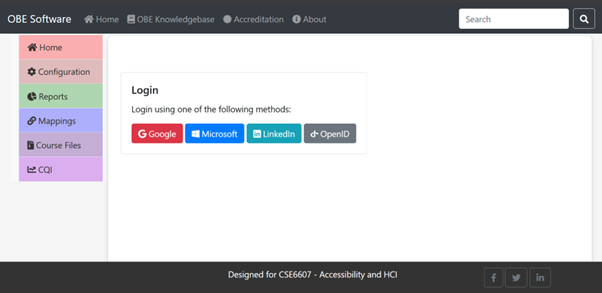
\includegraphics[width=0.8\linewidth]{img/Picture4.png}
    \caption{Pseudo interface for the OBE Software}
    \label{fig:pseudo-interface}
\end{figure}


\begin{itemize}
    
    \item \textbf{Top menu bar: }P3, P4, and P5 highlighted that the top menu bar should provide links to the publicly available documents relevant to OBE and accreditation. The search box in the top menu should suggest relevant terms. P3 suggested the integration of recommender systems to provide improved suggestions. All the participants agreed that contextual icons before the menu items would help the interface to be more intuitive. Furthermore, the links to the accessibility features (e.g., switching themes, language) could also be placed at the sticky top menu.
    

\item \textbf{Footer: }All the participants agreed that the social media icons are unnecessary in this context and could be removed. The footer section could contain P3 suggested placing a suggestion box and branding information in the footer. 

\item \textbf{Left Menu: The left menu was designed to be }floating, simple and responsive. However, the inclusion of contextual icons was mentioned by P3 to increase intuitiveness. 

\item \textbf{Dashboard:} The dashboard should contain the left menu items, which would be the first page the user sees after logging in. P3 and P7 suggested including breadcrumbs at the top of every page showing the hierarchy of the interfaces.  The suggestions are depicted in Figure \ref{fig:dashboard}.

\begin{figure}
    \centering
    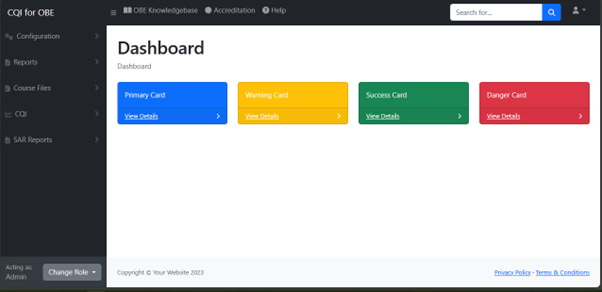
\includegraphics[width=0.8\linewidth]{img/Picture5.png}
    \caption{Sample Dashboard }
    \label{fig:dashboard}
\end{figure}

\item \textbf{Help Menu: }Instead of using a help menu, a contextual help icon, which would contain relevant information and instructions for the user could be displayed. This feature would require intelligence and could be implemented in future. 

\item \textbf{Institutional access: }All the participants agreed that an institutional login system could ease the accessibility and could provide better access control and privacy. 

\item \textbf{Accessibility features: }No specific recommendations were given by the participants for the accessibility features. However, during the semi structured interview, both P1 and P2 expressed their concerns about the accessibility features which were discussed earlier. 

\item \textbf{Social media buttons: }All the users agreed that the social media buttons are not that important for such a system. Hence the social media buttons from the footer section would be removed. 

\item \textbf{Additional recommendations: }

\begin{itemize}
    \item \textbf{Role-based interfaces:} P3 suggested using role-based interfaces, so that a faculty member can act as a course instructor, CQI committee member, or a Program Coordinator. Therefore, the functions offered to the user would be different based on the current role of the user. P3 also suggested that the change of roles could be placed at the bottom left corner of the screen, while logged in, as shown in Figure \ref{fig:roles}.

    \begin{figure}
        \centering
        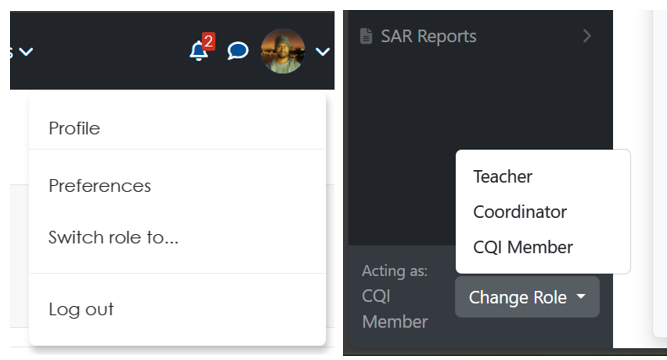
\includegraphics[width=0.8\linewidth]{img/Picture6.png}
        \caption{Changing roles}
        \label{fig:roles}
    \end{figure}
    
    \item \textbf{Historical Data Access:} P1 and P2 emphasized access of historical data for CQI interfaces for better data driven decision making. This feature was included in the user interface.
\end{itemize}
\end{itemize}






\subsubsection{\textbf{The CQI Module}}
\vspace{12pt}

The primary goal for CQI is self-explanatory, which is continuous improvement of quality. For benchmarking the education quality, historical access of data is critical. The CQI committee members are usually experts of OBE, having years of experience and training. Yet, the process necessitates data driven decision making, hence the CQI process must involve information from the past. 

\begin{figure}
    \centering
    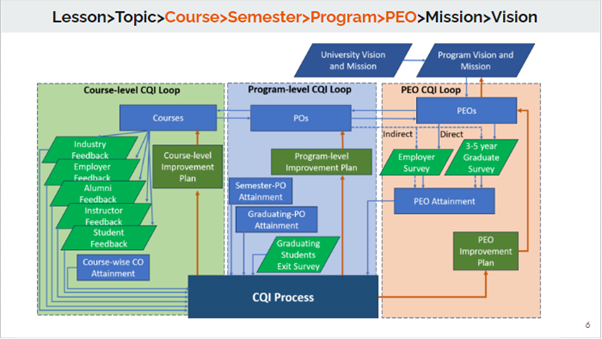
\includegraphics[width=0.8\linewidth]{img/Picture7.png}
    \caption{CQI Loops at different levels}
    \label{fig:cqi-loops}
\end{figure}
With different feedback loops as seen in Figure \ref{fig:cqi-loops}, data on student achievement (outcomes) are continuously collected and compared to program goals to adjust teaching methods, curriculum, or assessments in a cyclical process, ensuring ongoing improvement and alignment with desired learning outcomes.

\begin{itemize}
    \item \textbf{Overview of the CQI user interface: }
    
    The philosophy of CQI is to continuously track performance, and make data driven decisions. Hence the process involves monitoring and analyzing the impacts of previous improvement decisions, and suggesting improvement plans, based on the analysis. The CQI processes are divided into logical categories, such as Course level, Program level and Department level. At each level individual performance of a student needs to be tracked, as P1 suggested. Furthermore, for cohort assessments, aggregation of data would be required, based on various business logics, required to make the decisions.

For example, a course teacher would be interested to see the impacts of his previous decisions at the course level, or another teacher might be interested to see how his co-teachers were teaching, a teacher may want to improve CO2 attainment, and wants to see if the cohort set of students achieved CO2. Looking from the Program level, the department might want to see the collective performance of all the students of a particular course or batch. These business requirements would vary from institution to institution. Therefore, the CQI Interface would start with an overview of the overall CQI process, as shown in figure \ref{fig:CQI-Overview-page}. The participants were given a short overview for 12 handmade sketches of the primary outlook of the interface. The feedback was collected through interactive discussions and based on the suggestions; the design choices were made. 


\begin{figure}
    \centering
    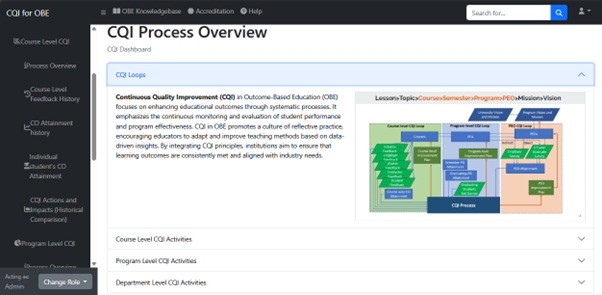
\includegraphics[width=0.8\linewidth]{img/Picture8.png}
    \caption{CQI Overview page}
    \label{fig:CQI-Overview-page}
\end{figure}




 \item \textbf{Course Level CQI Feedback History:}

Figure \ref{fig:Course-Level-CQI-Feedback-Historyl} demonstrates the UI for the Course Level CQI Feedback History. The initial plan was to be able search a particular course using a key, such that YYYY-S-XXXXXX-ZZ, where YYYY is the 4 digit year, \(S=\{1,2,3\} \rightarrow \{\text{Spring, Summer, Fall}\}\), followed by XXXXXX is a 6 digit course code and ZZ is a two digit section code. Such searching is faster for experienced CQI members. For example, \textit{CSE407 section 2} offered in \textit{Summer 2021} would have the key \textit{2021-2-CSE407-02}.

However, P3, P7 strongly suggested that such a key would be complicated to understand at first. Rather a series of dropdown and selection options could be incorporated. Tabs were included instead of creating separate pages, for compact view and less scrolling. This recommendation was appreciated by all the participants. 

\begin{figure}
    \centering
    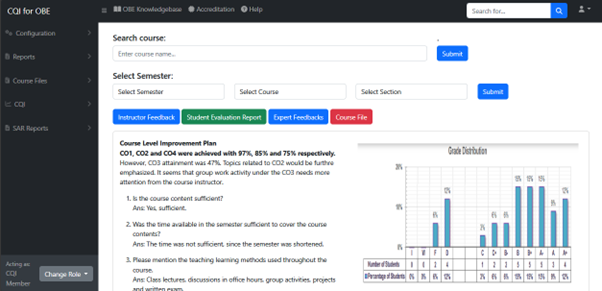
\includegraphics[width=0.8\linewidth]{img/Picture9.png}
    \caption{Course Level CQI Feedback History}
    \label{fig:Course-Level-CQI-Feedback-Historyl}
\end{figure}

Furthermore, each of the pages would have pictorial representations of the data for better comprehension. Separate tabs for different kinds of stakeholders are included for compact viewing. In the course level feedback page, the instructor feedback, student evaluation report, expert feedback, and course files could be accessed. This data would be available for the CQI members as well as the faculty members teaching the same course, as P1 suggested. 

 \item \textbf{Course Level CQI Plan History: Actions vs. Impacts}

Figure \ref{fig:course-level-cqi-history} provides a summarized overview of the CO attainment history of all the sections. The course level CO attainment for a particular section could be selected. For compact viewing, collapsible accordions were used for compact viewing. All the participants agreed that such a compact view would facilitate action vs. impact analysis for the CQI process. P4 and P5 suggested that aggregated data from several courses could also be designed in a similar fashion.



 \item \textbf{Program Level CQI: Feedback and Survey Results}

The program level CQI could involve both qualitative and quantitative data in the form of feedback, surveys, and quantitative analysis from the course level data. Since the feedback and surveys are not done after every semester, the timeframe of data collection would be mentioned. For example, Figures \ref{fig:program-level-cqi-feedbacks-survey} and \ref{fig:po-attainment} demonstrate the feedback and survey results for the 2023 Spring semester. Furthermore, P3, P6 and P7 suggested that the stakeholder feedback should also be timestamped.
\begin{figure}
    \centering
    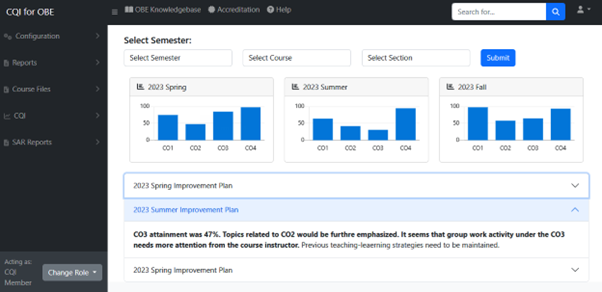
\includegraphics[width=0.8\linewidth]{img/Picture10.png}
    \caption{Course Level CQI History}
    \label{fig:course-level-cqi-history}
\end{figure}

\begin{figure}
    \centering
    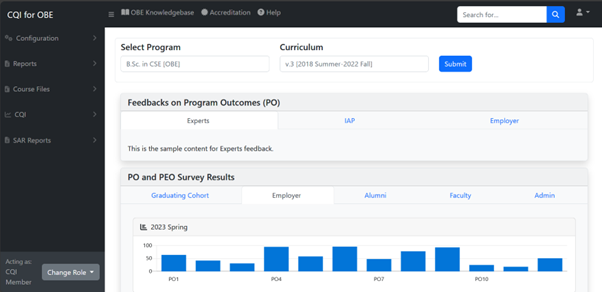
\includegraphics[width=0.8\linewidth]{img/Picture11.png}
    \caption{Program Level CQI Feedbacks and Survey Results}
    \label{fig:program-level-cqi-feedbacks-survey}
\end{figure}
\begin{figure}
    \centering
    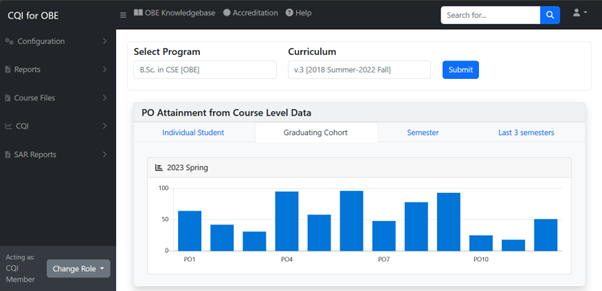
\includegraphics[width=0.8\linewidth]{img/Picture12.png}
    \caption{PO Attainment from course level quantitative data}
    \label{fig:po-attainment}
\end{figure}






   
\end{itemize}







 \subsection{\textbf{Limiting the scope of the project}}
 
The designed pages could be categorized as “Reports” of different kinds, containing historical data in the forms of texts, and charts. Utilizing the containerized design, any kind of report would be possible to create. P3 advocated for creating a report builder module with JavaScript for a drag-and-drop interface. 

The collected feedback indicates that information displayed on the pages should be shown in such a way that a decision could be taken at a glance. Inclusion of historical data was emphasized by almost all the participants during the interviews. Furthermore, the participants did not agree on designing a mobile interface, since such a software would be used in a professional environment, mostly on desktop computers. Frequency of usage of the program level CQI pages would not be more than course level pages. Therefore, P6 and P7 strongly argued in favor of having a mobile interface for the students and teachers modules, considering the frequency of access, and the user patterns. Considering the scope of the project, the editable interfaces were not designed. The user interfaces for other roles such as teacher, student, alumni and so on, were also considered beyond the scope of the proejct. 

The demographic details of the participants could have been diversified, including CQI committee members from different universities. However, UI design choices are subjective and heavily dependent on opinions. The compactness of the information display could be overwhelming and may demand a simpler static webpage. For printing the data, simpler static web pages could be generated instantly using accessibility tools. 

\subsection{Comparison with commercial solutions}
 There are a number of commercial solutions that offer similar services. However, P4 and P5 were not CQI members of the commercial solution, hence the comparison is due. Furthermore, internationally available solutions are custom made and did not offer any of the modules that had been discussed by the developers. The researcher himself attended a number of commercial sales demonstrations of IonCUDOS and UCAM, both being widely used at home and abroad. UCAM is a locally made commercial solution provided by Edusoft Consultants Ltd., and often were considered unaffordable due to financial constraints. 


 
\section{\textbf{Ethical Considerations}}
 All the participants were informed much earlier about the interviews, with their prior consent. Approval from an Institutional Review Board (IRB) would be required for publishing the results in future. At this point, IRB approval was not taken. 

\section{\textbf{Discussion}}

\begin{itemize}
    \item \textbf{Drivers and Barriers of OMS Development}


The development and implementation of outcomes measurement software (OMS) in Outcome-Based Education (OBE) for undergraduate engineering programs in Bangladesh are influenced by multiple factors that span institutional commitments, technological advancements, educational philosophies, and stakeholder perspectives.

Key drivers motivating the development of OMS in the context of OBE include the principles of constructive alignment and skills-based learning. These principles emphasize the importance of aligning educational objectives, teaching methods, and assessments to ensure students acquire the necessary skills and competencies. OMS is perceived as a critical tool to facilitate this alignment by providing a structured platform for tracking student progress, assessing achievement levels, and monitoring cohort performance. Institutional commitments to quality education and global competitiveness further drive the development and adoption of OMS. Technological advancements, particularly in information technology, are leveraged to make OMS more accessible and user-friendly.

However, despite these drivers, several barriers and challenges hinder the successful implementation of OMS in undergraduate engineering programs within the Bangladesh higher education system. Financial constraints, technological challenges, and institutional cultures manifest as significant obstacles towards the implementation of OMS. Budget limitations often restrict the scope and scale of OMS development, while technological challenges, such as the lack of skilled personnel and infrastructure, impede the effective utilization of OMS. Institutional cultures that resist change and innovation further complicate the integration of OMS into existing educational practices.

Distinct perspectives of university administrators and faculty members shed light on the complexities surrounding the development and implementation of OMS. University administrators emphasize the importance of OMS in enhancing institutional reputation, ensuring accreditation compliance, and fostering continuous improvement in educational quality. On the other hand, faculty members perceive OMS as a valuable tool for improving teaching methodologies, facilitating data-driven decision-making, and enhancing student assessment practices. However, concerns regarding the learning curve, resistance to change, and the potential for increased workload are also voiced by faculty members.

Accessibility features and assistive technologies for visually impaired people are crucial considerations in the development and implementation of OMS. Voice-assisted technologies, high contrast modes, and screen reading capabilities are among the most crucial accessibility features that need to be integrated into OMS to ensure inclusivity and equitable access to educational resources and opportunities for visually impaired individuals.

Based on the identified drivers and challenges, strategic recommendations can be proposed for optimizing the development and implementation of OMS in the context of OBE for undergraduate engineering students. An agile development approach, stakeholder engagement, capacity building, and professional development initiatives are recommended to address the identified barriers effectively. Actionable recommendations to overcome challenges and ensure the successful integration of OMS include fostering a culture of innovation, promoting collaborative partnerships, leveraging existing resources, and aligning OMS development with institutional goals and priorities.

Interviews revealed a number of underlying driving factors and hurdles in the context of OBE software development. It is evident from the study that the underlying reasons originate from several domains that influence the adoption of assistive technologies for education. Theoretical analysis based on TAM and UTAUT frameworks also reveal that the factors range from social, cultural, financial categories. While the experienced participants were found to be more flexible with the design choices.

One important issue is there are no specific guidelines for software usage for OBE. Nor are there any requirements imposed by BAETE for accreditation. OBE practices in organizations that just started would not be as detailed as the experienced organizations. Furthermore, implementing any change at the institutional level would require a series of approvals from the higher authorities which is time consuming. Therefore the design choices need to be analyzed thoroughly before final implementation, keeping organizational culture in mind. 

\item \textbf{Human-Computer Interaction (HCI) in Outcome-Based Education (OBE) Software}

Human-Computer Interaction (HCI) plays a critical role in the successful development and implementation of outcomes measurement software (OMS) within the context of Outcome-Based Education (OBE) for undergraduate engineering programs. HCI focuses on the design and usability of computer systems, ensuring that they are intuitive, efficient, and user-friendly. In the context of OMS for OBE, effective HCI principles are essential for facilitating the interaction between users and the software, optimizing workflow efficiency, and enhancing overall user experience.

One of the primary objectives was to create interfaces that enable seamless navigation and interaction with the OMS platform. Given the diverse stakeholders, which includes faculty members, administrators, and students, the interface must accommodate varying levels of technological proficiency and preferences. Intuitive navigation systems, clear labeling, and consistent design elements are crucial for ensuring that users can easily access and utilize the features and functionalities of the OMS platform.

Moreover, HCI principles guided the design of interfaces that support the specific workflow requirements of OBE implementation. For example, in the Continuous Quality Improvement (CQI) module, interfaces are designed to facilitate data-driven decision-making processes by providing users with access to historical data, feedback mechanisms, and analysis tools. The design of the CQI interface incorporates feedback loops and visual representations of data to support iterative improvement cycles and enable stakeholders to make informed decisions about curriculum, teaching methods, and assessments.

Additionally, the design of accessibility features within the OMS platform, ensuring inclusivity and equitable access to educational resources for all users, including those with disabilities. Features such as voice-assisted technologies, high contrast modes, and screen reading capabilities, could be integrated to accommodate visually impaired users and enhance accessibility.

Iterative design processes, user feedback, and usability testing are integral components in OBE implementation. By soliciting feedback from users and conducting usability tests, developers can identify usability issues, refine interface designs, and optimize user workflows. The interactive design process involved stakeholders in the design decision-making process, ensuring that the final product meets their needs and expectations.

Furthermore, the interfaces support collaboration and knowledge sharing among users. In the context of OBE, where collaborative learning and continuous improvement are emphasized, interfaces that facilitate communication, document sharing, and collaborative decision-making are essential. For example, features such as shareable course contents, collaborative course planning tools, and interactive feedback mechanisms promote collaboration among faculty members and administrators, fostering a culture of continuous improvement and innovation in OBE implementation.

By integrating principles of usability, accessibility, workflow optimization, and collaboration, the goal was to make the OMS platform user-centric, efficient, and effective for supporting OBE practices. As OBE continues to evolve and adapt to changing educational landscapes, HCI will remain a cornerstone in the design and enhancement of OMS platforms, enabling stakeholders to achieve their educational goals and objectives effectively. 
\end{itemize}
\section{\textbf{Conclusion}}
OBE software could act as an assistive technology for the adoption of Outcome Based Education in Bangladesh. Considering the socio-cultural contexts, a number of barriers would be faced for implementing such a system, however, the driving factors are also strong for OBE adoption. Considering complex functionalities, ever-changing requirements, differences in mindsets and practices, development of an in-house solution seems to be the best choice in hand. However, organizations could coordinate the development, integration and adoption of such a software by assigning a dedicated team or person to be responsible for the OBE software. The UTAUT did not reveal much about age, gender being much influential, rather ease of use and performance expectancy were perceived to be crucial for the experienced users. The CQI module is the heart of OBE which requires the CQI committee members to be able to view the required information readily with ease with a compact view. The design choices were adjusted according to the feedback received and positive feedback affirm the philosophy of compact UI design with less scrolling. In conclusion, while user-friendliness is key for widespread adoption, a custom-developed OBE software can address the specific needs and complexities of Bangladeshi educational institutions.  A dedicated team can oversee development and ensure the software effectively supports OBE implementation.

\vspace{\baselineskip}


Weblink: \href{https://modules.ewubd.edu/obepages/static-pages}{https://modules.ewubd.edu/obepages/static-pages}
\newline
\vspace{\baselineskip}
Interview transcripts, sketches are available in the Appendices. 

 



% if have a single appendix:
%\appendix[Proof of the Zonklar Equations]
% or
%\appendix  % for no appendix heading
% do not use \section anymore after \appendix, only \section*
% is possibly needed

% use appendices with more than one appendix
% then use \section to start each appendix
% you must declare a \section before using any
% \subsection or using \label (\appendices by itself
% starts a section numbered zero.)
%


%\appendices
%\section{section title}

% you can choose not to have a title for an appendix
% if you want by leaving the argument blank
%\section{}



% use section* for acknowledgment
%\section*{Acknowledgment}





% Can use something like this to put references on a page
% by themselves when using endfloat and the captionsoff option.
\ifCLASSOPTIONcaptionsoff
  \newpage
\fi



% trigger a \newpage just before the given reference
% number - used to balance the columns on the last page
% adjust value as needed - may need to be readjusted if
% the document is modified later
%\IEEEtriggeratref{8}
% The "triggered" command can be changed if desired:
%\IEEEtriggercmd{\enlargethispage{-5in}}

% references section

% can use a bibliography generated by BibTeX as a .bbl file
% BibTeX documentation can be easily obtained at:
% http://mirror.ctan.org/biblio/bibtex/contrib/doc/
% The IEEEtran BibTeX style support page is at:
% http://www.michaelshell.org/tex/ieeetran/bibtex/
%\bibliographystyle{IEEEtran}
% argument is your BibTeX string definitions and bibliography database(s)
%\bibliography{IEEEabrv,../bib/paper}
%
% <OR> manually copy in the resultant .bbl file
% set second argument of \begin to the number of references
% (used to reserve space for the reference number labels box)


\bibliographystyle{IEEEtran}
\bibliography{paper}



% biography section
% 
% If you have an EPS/PDF photo (graphicx package needed) extra braces are
% needed around the contents of the optional argument to biography to prevent
% the LaTeX parser from getting confused when it sees the complicated
% \includegraphics command within an optional argument. (You could create
% your own custom macro containing the \includegraphics command to make things
% simpler here.)
%\begin{IEEEbiography}[{\includegraphics[width=1in,height=1.25in,clip,keepaspectratio]{mshell}}]{Michael Shell}
% or if you just want to reserve a space for a photo:



% You can push biographies down or up by placing
% a \vfill before or after them. The appropriate
% use of \vfill depends on what kind of text is
% on the last page and whether or not the columns
% are being equalized.

%\vfill

% Can be used to pull up biographies so that the bottom of the last one
% is flush with the other column.
%\enlargethispage{-5in}



% that's all folks
\end{document}